\documentclass{article}
\usepackage{geometry}
\usepackage{amsmath, amssymb, amsthm}
\usepackage{lmodern}
\usepackage{tikz}
\usetikzlibrary{positioning}

\usepackage[
backend=biber,
style=alphabetic,
sorting=ynt
]{biblatex}
\addbibresource{refs.bib}

\title{
\vspace{-2.5cm}
A research proposal for the computational complexity of
minimizing reducible sofic shifts
}
\author{Justin Cai}

\newcommand{\Ac}{\mathcal{A}}  % alphabet
\newcommand{\Fc}{\mathcal{F}}
\newcommand{\Lc}{\mathcal{L}}  % label function
\newcommand{\Gc}{\mathcal{G}}  % labeled graph
\newcommand{\Hc}{\mathcal{H}}  % labeled graph
\newcommand{\Vc}{\mathcal{V}}
\newcommand{\Ec}{\mathcal{E}}
\newcommand{\Bc}{\mathcal{B}}
\newcommand{\shift}[1]{\mathsf{X}_{#1}}
\newcommand{\term}[1]{\textit{#1}}

\newtheorem{theorem}{Theorem}
\newtheorem{definition}{Definition}
\newtheorem*{question}{Question}
% \newtheorem{example}{Example}

\begin{document}

\maketitle

\begin{abstract}
    In symbolic dynamics, a certain class of objects 
    called sofic shifts are sets of bi-infinite
    sequences that come from labeled graphs, such that each letter of 
    the sequence is the label of an edge in a bi-infinite walk around the graph.
    If one wanted to use sofic shifts to model something, it would be desirable to 
    have a graph that is as small as it can be while still presenting the same sequences.
    While the problem of how hard it is to compute this minimal graph for shifts with a 
    certain property called irreducibility is known, the hardness of computing the same
    problem for shifts that do not have this property is unknown.
\end{abstract}

\section{Background}

% Symbolic dynamics studies a class of bi-infinite sequences over a finite alphabet called 
% shift spaces; such spaces have the property of being shift invariant.

% A bi-infinite sequence over a finite alphabet \(\Ac\) is an assignment of a symbol
% from \(\Ac\) to each integer. Such sequences 

% In symbolic dynamics, the \term{full shift} \(\Ac^\mathbb{Z}\) is the collection of 
% all bi-infinite sequences over symbols from a finite alphabet \(\Ac\).
% Elements from the full shift are called a points. For a point \(x\) from the full shift,
% we can denote it \[x=(x_i)_{i \in \mathbb{Z}} = \hdots x_{-2} x_{-1} x_0 x_1 x_2 \hdots,\]
% where \(x_i\) is the \term{\(i\)th coordinate} of \(x\). Hence, a point is defined by assigning 
% each coordinate with a symbol from the alphabet.
% A \term{block}
% (or \term{word}) is a finite sequence of symbols from \(\Ac\). The block starting
% at the \(i\)th coordinate and ending at the \(j\)th coordinate
% is denoted \(x_{[i,j]}=x_i x_{i+1} \hdots x_{j}\). A block \(w\) \term{occurs} in \(x\)
% if there exists \(i,j \in \mathbb{Z}\) such that \(x_{[i,j]}=w\). For a collection
% of blocks \(\Fc\) over \(\Ac\), define \(\shift{\Fc}\) to be the subset of points in \(\Ac^\mathbb{Z}\) 
% such that every block in \(\Fc\) does not occur in \(x\). Finally, a \term{shift space} is a 
% subset \(X\) of the full shift such that there exists a collection \(\Fc\) such that \(X = \shift{\Fc}\).

% Let's look at some examples of shift spaces. For these examples, we'll consider sets 
% of sequences of Let \(X\) be the set of all 

A \term{full shift} is the set of all bi-infinite sequences over a finite alphabet \(\Ac\).
A \term{graph} \(G\) is a finite set of \term{verticies} \(\Vc=\Vc(G)\) and a finite set 
of edges \(\Ec = \Ec(G)\) with each edge \(e\) starting at a vertex \(i(e) \in \Vc\)
and terminating at a vertex \(t(e) \in \Vc\). 
A bi-infinite walk on \(G\) is a bi-infinite sequence of edges such that the 
terminating vertex of each edge is the inital vertex of the next edge. The set of 
all bi-infinite walks on \(G\) is called the \term{edge shift} \(\shift{G}\).
A \term{labeled graph} \(\Gc\)
is a graph \(G\) equipped with a \term{labeling} \(\Lc: \Ec(G) \to \Ac\), which assigns each
edge \(e\) from \(G\) a label \(\Lc(e)\) from a finite alphabet \(\Ac\). If \(x\) is 
a bi-infinite walk on \(G\), then the \term{label of the walk} \(\Lc_\infty(x)\) is 
the bi-infinite sequence of the labels of \(x\). The set of all labels of bi-infinite 
walks is denoted \(\shift{\Gc}\). A subset \(X\) of a full shift is a \term{sofic shift} if \(X = \shift{\Gc}\)
for some labeled graph \(\Gc\). A labeled graph \(\Gc\) is a \term{presentation} 
of \(X\) if \(X=\shift{\Gc}\).

For example, let \(X\) be the set of bi-infinite sequences over \(\{0,1\}\) such that 
there is an even number of \(0\)'s between any two \(1\)'s. Then \(X=\shift{\Gc}\), where
\(\Gc\) is any labeled graph in Figure 1. This shift is known as the \term{even shift}.
\begin{figure}[h]
    \centering
    \begin{tikzpicture}
        \node[shape=circle, draw=black] (A) at (0,0) {};
        \node[shape=circle, draw=black] (B) at (2,0) {};

        \path [->] (A) edge[out=225, in=135, distance=10mm] node[left] {$1$} (A);
        \path [->] (A) edge[out=45, in=135] node[above] {$0$} (B);
        \path [->] (B) edge[out=225, in=-45] node[below] {$0$} (A);

        \node[shape=circle, draw=black] (A) at (4,-1) {};
        \node[shape=circle, draw=black] (B) at (6,-1) {};
        \node[shape=circle, draw=black] (C) at (6,1) {};
        \node[shape=circle, draw=black] (D) at (4,1) {};

        \path[->] (A) edge[out=180, in=-90, distance=10mm] node[left] {$1$} (A);
        \path[->] (C) edge[out=0, in=90, distance=10mm] node[right] {$1$} (C);
        \path[->] (A) edge node[below] {$0$} (B);
        \path[->] (B) edge node[right] {$0$} (C);
        \path[->] (C) edge node[above] {$0$} (D);
        \path[->] (D) edge node[left] {$0$} (A);

        \node[shape=circle, draw=black] (A) at (8.5, 0) {};
        \node[shape=circle, draw=black] (B) at (10.5, -1) {};
        \node[shape=circle, draw=black] (C) at (10.5, 1) {};

        \path[->] (A) edge[out=135, in=-135, distance=10mm] node[left] {$1$} (A);
        \path[->] (A) edge node[below] {$1$} (B);
        \path[->] (B) edge[out=60, in=-60] node[right] {$0$} (C);
        \path[->] (C) edge[out=-120, in=120] node[left] {$0$} (B);
        \path[->] (C) edge node[above] {$0$} (A);

    \end{tikzpicture} 
    \caption{Presentations of the even shift}
\end{figure}

\newpage

A \term{block} is a finite sequence of symbols over an alphabet. Let \(x\) be a point 
from a sofic shift. We way the a block \(w\) \term{occurs} in \(x\) if there exists 
integers \(i, j\) such that \(x_i x_{i+1} \hdots x_{j} = w\). The \term{language} of a 
sofic shift \(\Bc(X)\) is the collection of blocks that occur in any point in \(X\).
A sofic shift is \term{irreducible} if for any pair of blocks \(u,v \in \Bc(X)\), there 
exists another block \(w \in \Bc(X)\) such that \(uwv \in \Bc(X)\).

A presentation is \term{right-resolving} if for each vertex in the presentation, the 
labels of the outgoing edges of that vertex are all distinct. For example, the left and middle graphs 
in Figure 1 are right-resolving while the right graph is not right-resolving. A graph 
is \term{irreducible} if for each pair of vertices, there exists a path in the graph 
from the first vertex to the second vertex and path from the second vertex to the first vertex.
Each graph in Figure 1 is irreducible.

For a labled graph, the \term{follower set} is the set of labels of the paths 
that 

A \term{minimal right-resolving} presentation of a sofic shift \(X\) is a 
right-resolving presentation of \(X\) having the fewest vertices among all 
right-resolving presentations of \(X\). 

\section{Minimization of reducible presentations}


From \cite{lind1995introduction} corollary (3.3.20), from an irreducible right-resolving
presentation, we can find the minimal right-resolving presentation by merging 
vertices in the presentation that have the same follower set, creating a 
follower-seperated presentation. However, this does not work for reducible graphs, as 
being follower-separated does not imply minimality. We can see this with this presentation 
of the even shift:

\begin{figure}[h]
    \centering
    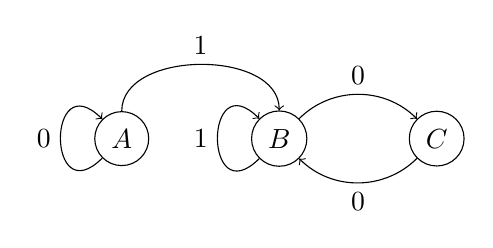
\begin{tikzpicture}
        \node[shape=circle, draw=black] (A) at (0,0) {\(B\)};
        \node[shape=circle, draw=black] (B) at (2,0) {\(C\)};
        \node[shape=circle, draw=black] (C) at (-2,0) {\(A\)};

        \path [->] (A) edge[out=225, in=135, distance=10mm] node[left] {$1$} (A);
        \path [->] (A) edge[out=45, in=135] node[above] {$0$} (B);
        \path [->] (B) edge[out=225, in=-45] node[below] {$0$} (A);
        \path [->] (C) edge[out=90, in=90] node[above] {$1$} (A);
        \path [->] (C) edge[out=225, in=135, distance=10mm] node[left] {$0$} (C);

    \end{tikzpicture} 
    \caption{A reducible, follower-separated presentation of the even shift}
\end{figure}

The block \(01\) does not appear in the follower set of \(B\), but does for the follower 
set of \(A\), so \(F_\Gc(A) \ne F_\Gc(B)\). The follower set of \(C\) is distinct from
the follower sets of \(A\) and \(B\), as any word that starts with \(1\) that appears in 
\(F_\Gc(A)\) and \(F_\Gc(B)\) does not appear in \(F_\Gc(C)\), so \(F_\Gc(A) \ne F_\Gc(C)\) and 
\(F_\Gc(B) \ne F_\Gc(C)\). Hence, the graph is follower-separated. This graph also presents 
the even shift. The label of any bi-infinite walk that visits \(A\) has the left-infinite 
sequence of an infinite number of \(0\)'s, followed by a \(1\), and then followed by a 
right-infinite sequence from the even shift. Since an infinite number of \(0\)'s followed by 
a \(1\) is a left-infinite sequence for the even shift, a walk visiting \(A\) is in the 
even shift. Any walk only visiting \(B\) and \(C\) is also a walk in the even shift. 

\begin{question}
    What are necessary and sufficient conditions for minimal, reducible, right-resolving graphs 
    
\end{question}

\printbibliography

\end{document}